%%%%%%%%%%%%%%%%%%%%%%%%%%%%%%%%%%%%%%%%%%%%%%%%%%%%%%%%%%%
% Szablon ksi��ki
% Autor: Tomasz Kubik
% udost�pniany na prawach CreativeCommons: SA-BY-NC
%
%%%%%%%%%%%%%%%%%%%%%%%%%%%%%%%%%%%%%%%%%%%%%%%%%%%%%%%%%%%
\documentclass[a4paper,11pt,polish]{memoir}
% acelnosxz
% ����󶼿
% ��ʣ�Ӧ��
%%%%%%%%%%%%%%%%%%%%%%%%%%%%%%%%%%%%%%%%%%%%%%%%%%%%%%%%%%%%
%%    Pakiety podstawowe                                  %%
%%%%%%%%%%%%%%%%%%%%%%%%%%%%%%%%%%%%%%%%%%%%%%%%%%%%%%%%%%%%
\usepackage[cp1250]{inputenc} %ustawienie kodowania znak�w
\usepackage[T1]{fontenc}
\usepackage{pslatex}
\usepackage[polish]{babel}
\usepackage{tabularx}
\usepackage{multicol}
\usepackage{color,colortbl}
\usepackage{calc,soul,fourier}
\usepackage{setspace}
\usepackage{indentfirst}
\usepackage{type1cm,eso-pic}
\usepackage{ifpdf}
\usepackage{amsmath}  
\usepackage{listings}
\usepackage{longtable}

%%%%%%%%%%%%%%%%%%%%%%%%%%%%%%%%%%%%%%%%%%%%%%%%%%%%%%%%%%%%
%%    Pakiety dodatkowe                                   %%
%%%%%%%%%%%%%%%%%%%%%%%%%%%%%%%%%%%%%%%%%%%%%%%%%%%%%%%%%%%%
%\RequirePackage[caption=false,position=bottom]{subfig} 
%\let\subbottom\subfloat
%\usepackage[version=3]{mhchem}

%%%%%%%%%%%%%%%%%%%%%%%%%%%%%%%%%%%%%%%%%%%%%%%%%%%%%%%%%%%%
%%    Pakiety do bibliografii i importu grafiki           %%
%%%%%%%%%%%%%%%%%%%%%%%%%%%%%%%%%%%%%%%%%%%%%%%%%%%%%%%%%%%%
\usepackage[sectionbib]{chapterbib}
\makeatletter
\renewcommand{\@memb@bsec}{\section*{\bibname}\prebibhook}
\makeatother

\usepackage{makeidx} \makeindex 
\ifpdf
 \usepackage[pdftex,bookmarks,breaklinks,unicode]{hyperref}
 \usepackage[pdftex]{graphicx}
 \DeclareGraphicsExtensions{.pdf,.jpg,.mps,.png}
 \pdfcompresslevel=9
\else
 \usepackage{graphicx}
 \DeclareGraphicsExtensions{.eps,.ps,.jpg,.mps,.png}
\fi

%%%%%%%%%%%%%%%%%%%%%%%%%%%%%%%%%%%%%%%%%%%%%%%%%%%%%%%%%%%%
%%    Znaczniki ci�cia                                    %%
%%%%%%%%%%%%%%%%%%%%%%%%%%%%%%%%%%%%%%%%%%%%%%%%%%%%%%%%%%%%
\makeatletter
\AddToShipoutPicture{%
  \setlength{\unitlength}{1mm}
%% 162 x 234
  \put(18,31.5){\line(-1,0){10}}%29.5
  \put(24,26.5){\line(0,-1){10}}%21
  \put(192,31.5){\line(1,0){10}}%29.5
  \put(186,26.5){\line(0,-1){10}}%189
  \put(18,265.5){\line(-1,0){10}}%267.5
  \put(24,270.5){\line(0,1){10}}%21
  \put(192,265.5){\line(1,0){10}}%267.5
  \put(186,270.5){\line(0,1){10}}%189
%% 168 x 238
 \put(18,29.5){\line(-1,0){10}}%
  \put(21,26.5){\line(0,-1){10}}%
  \put(192,29.5){\line(1,0){10}}%
  \put(189,26.5){\line(0,-1){10}}%
  \put(18,267.5){\line(-1,0){10}}%
  \put(21,270.5){\line(0,1){10}}%
  \put(192,267.5){\line(1,0){10}}%
  \put(189,270.5){\line(0,1){10}}%
}
\makeatother

%%%%%%%%%%%%%%%%%%%%%%%%%%%%%%%%%%%%%%%%%%%%%%%%%%%%%%%%%%%%
%%    Ustawienia strony + definicje pomocnicze            %%
%%%%%%%%%%%%%%%%%%%%%%%%%%%%%%%%%%%%%%%%%%%%%%%%%%%%%%%%%%%%
\setlength{\headsep}{9pt} 
%\setlength{\headheight}{0pt}
\setlength{\hoffset}{0mm} %%a4
\setlength{\voffset}{0mm} %-14mm %%a4
\setlength{\footskip}{23pt} % 23pt ~= 8mm
\setlength{\topmargin}{13mm}%{7.65mm} %28pt -2.5mm
%\setlength{\oddsidemargin}{11.85mm}
%\setlength{\evensidemargin}{11.85mm}
%\setlength{\textwidth}{135.5mm}
%\setlength{\textheight}{203.6mm}

\setlength{\parindent}{15pt}
\setlength{\parskip}{0pt} %{1ex plus 0.5ex minus 0.2ex}
\newlength\mytemplengtha

\setlength{\extrarowheight}{2pt}
%\setlength{\topmargin}{8mm}%{7.65mm} %28pt -2.5mm
\setlength{\oddsidemargin}{15mm}
\setlength{\evensidemargin}{15mm}
\setlength{\textwidth}{129mm}%135.5
\setlength{\textheight}{201mm}%203.6
%\setlength{\parindent}{16pt}%18


\sloppy  % wyr�wnanie z dw�ch stron
\renewcommand{\topfraction}{1.0}
\renewcommand{\bottomfraction}{1.0}
\renewcommand{\textfraction}{0.0}

\widowpenalty=10000 % ostatni wiersz akapitu nie zostanie przeniesiony na nast?pn? stron? 
\clubpenalty=10000 % pierwszy wiersz akapitu nie b?dzie ko?czy? strony (nie u?ywam tego ustawienia)
%\tolerance = 500 \pretolerance = 900 %% sk?ad z wi?ksz? `tolerancj?' (mo?na te warto?ci zwi?kszy? bardziej)
%\hbadness= 1450 %% zmniejsza licz? wy?wietlanych ostrze?e? (mo?na zwi?kszy?, ale bez przesady)
%\hfuzz = 1.5pt %% tekst mo?e stercze? ma marginesie na 1,5pt (ok. 0,5mm)

\setlength\floatsep{6pt plus 2pt minus 2pt} 
\setlength\intextsep{12pt plus 2pt minus 2pt} 
\setlength\textfloatsep{12pt plus 2pt minus 2pt} 
%\captionnamefont{\small\bfseries}
%\captiontitlefont{\small}
\setbeforesecskip{10pt plus 0.5ex}%{-3.5ex \@plus -1ex \@minus -.2ex}
\setaftersecskip{10pt plus 0.5ex}%\onelineskip}
\setbeforesubsecskip{8pt plus 0.5ex}%{-3.5ex \@plus -1ex \@minus -.2ex}
\setaftersubsecskip{8pt plus 0.5ex}%\onelineskip}

%\setlength{\floatsep}{12pt}
%\setlength{\textfloatsep}{12pt}
%\setlength{\intextsep}{12pt}
%\setlength{\arrayrulewidth}{0.5pt}
\usepackage{color}
\definecolor{lightgray}{rgb}{.9,.9,.9}
\definecolor{darkgray}{rgb}{.4,.4,.4}
\definecolor{purple}{rgb}{0.65, 0.12, 0.82}
%\definecolor{nicered}{rgb}{.647,.129,.149}
\definecolor{nicered}{rgb}{.0,.0,.0}

%%%%%%%%%%%%%%%%%%%%%%%%%%%%%%%%%%%%%%%%%%%%%%%%%%%%%%%%%%%%
%%    Zmienione otoczenia                                 %%
%%%%%%%%%%%%%%%%%%%%%%%%%%%%%%%%%%%%%%%%%%%%%%%%%%%%%%%%%%%%
\makeatletter
\renewenvironment{itemize}{
  \begin{list}{  
  \csname labelitem\romannumeral\the\@listdepth\endcsname}{
  \setlength{\leftmargin}{1em}
	\setlength{\topsep}{6pt}%
	\setlength{\partopsep}{0pt}%
	\setlength{\parskip}{0pt}%
	\setlength{\parsep}{0pt}%
	\setlength{\itemsep}{0pt}}
}{
  \end{list}
}
\renewenvironment{quote}{
  \begin{list}{}{}
	 \item[]}
	 {\unskip\end{list}}
\makeatother

\setlength{\leftmargini}{1.5em}
\usepackage{bibspacing}
\setlength{\bibspacing}{\baselineskip}

\makeatletter
\newskip\@hlskip
%\@hlskip=.5\baselineskip \@plus 1mm \@minus .5mm
\@hlskip=6pt

\newdimen\verbatimleftmargin
  \verbatimleftmargin\z@
\newdimen\verbatimbaselineskip
  \verbatimbaselineskip\baselineskip
\def\verbatimsize{\normalsize}

\def\@verbatim{%
 \topsep\@hlskip
 \partopsep\z@\parsep\z@\itemsep\z@
 \trivlist \item\relax
  \if@minipage\else
   \vskip\baselineskip
   \vskip-\verbatimbaselineskip
%  \vskip\parskip
  \fi
  \leftskip\@totalleftmargin
  \if@minipage\else
   \advance \leftskip by \verbatimleftmargin
  \fi
  \rightskip\z@skip
  \parindent\z@\parfillskip\@flushglue\parskip\z@skip
  \@@par
  \@tempswafalse
  \def\par{%
    \if@tempswa
      \leavevmode \null \@@par\penalty\interlinepenalty
    \else
      \@tempswatrue
      \ifhmode\@@par\penalty\interlinepenalty\fi
    \fi}%
  \let\do\@makeother \dospecials
  \obeylines 
   \verbatimsize \baselineskip\verbatimbaselineskip
   \verbatim@font \@noligs
  \everypar \expandafter{\the\everypar \unpenalty}%
}
\makeatother


\newcommand{\autorzy}{}

\makeatletter
\newlength\dlf@normtxtw
\setlength\dlf@normtxtw{\textwidth}
\def\myhelvetfont{\def\sfdefault{mdput}}
\newsavebox{\feline@chapter}
\newcommand\feline@chapter@marker[1][4cm]{%
\sbox\feline@chapter{%
\resizebox{!}{#1}{\fboxsep=1pt%
\colorbox{nicered}{\color{white}\bfseries\sffamily\thechapter}%
}}%
\rotatebox{90}{%
\resizebox{%
\heightof{\usebox{\feline@chapter}}+\depthof{\usebox{\feline@chapter}}}%
{!}{\scshape\so\@chapapp}}\quad%
\raisebox{\depthof{\usebox{\feline@chapter}}}{\usebox{\feline@chapter}}%
}
\newcommand\feline@chm[1][4cm]{%
\sbox\feline@chapter{\feline@chapter@marker[#1]}%
\makebox[0pt][l]{% aka \rlap
\makebox[1cm][r]{\usebox\feline@chapter}%
}}
\makechapterstyle{daleif1}{
\renewcommand\chapnamefont{\normalfont\Large\scshape\raggedleft\so}
\renewcommand\chaptitlefont{\normalfont\huge\bfseries\scshape\color{nicered}}
\renewcommand\chapternamenum{}
\renewcommand\printchaptername{}
\renewcommand\printchapternum{\vspace{-3cm}\null\hfill\feline@chm[2.5cm]\par}
\renewcommand\afterchapternum{\par\vskip\midchapskip}
\renewcommand\printchaptertitle[1]{\chaptitlefont\raggedleft ##1\\  \makebox[\textwidth - (1cm + \widthof{\Huge \thechapter.})][r]{\Large \itshape \autorzy}\par}
}

\addtopsmarks{headings}{%
\nouppercaseheads % added at the beginning
}{%
\createmark{chapter} {left}{shownumber}{}{. \space}
\createmark{section}{right}{shownumber}{}{. \space}
}%use the new settings
\pagestyle{headings}

\setcounter{secnumdepth}{2}
\setcounter{tocdepth}{2}
\setsecnumdepth{subsection} % activating subsubsec numbering in doc


%definicja nag��wk�w
\copypagestyle{outer}{headings}
\makeoddhead{outer}{}{}{\small\color{nicered}\slshape\rightmark}
\makeevenhead{outer}{\small\color{nicered}\slshape\leftmark}{}{}
\makeoddfoot{outer}{}{}{\thepage}
\makeevenfoot{outer}{\thepage}{}{}
% fix plain
%\copypagestyle{plain}{outer} % overwrite plain with outer
\makeoddhead{plain}{}{}{} % remove right header
\makeevenhead{plain}{}{}{} % remove left header
\makeevenfoot{plain}{}{}{}
\makeoddfoot{plain}{}{}{}

\makepagestyle{intro}
\makeoddhead{intro}{}{}{\small\color{nicered}\slshape S�owo wst�pne}
\makeevenhead{intro}{\small\color{nicered}\slshape S�owo wst�pne}{}{}
\makeoddfoot{intro}{}{}{\thepage}
\makeevenfoot{intro}{\thepage}{}{}

%\renewcommand{\chaptermark}[1]{\markboth{\ifnum \c@secnumdepth >\z@ \thechapter \ \fi #1}{}} 
%\renewcommand{\chaptermark}[1]{\markboth{\thechapter \ #1}{\thesection \ #1}} 
%\renewcommand{\sectionmark}[1]{\markright{\thesection \ #1}{}} 
%\renewcommand{\chaptermark}[1]{\markboth{\thechapter \MakeUppercase{#1}}{}}

%kropki po numerach sekcji
\makeatletter
\def\@seccntformat#1{\csname the#1\endcsname.\quad}
\def\numberline#1{\hb@xt@\@tempdima{#1\if&#1&\else.\fi\hfil}}
\makeatother

% z jakiego? powodu czcionki s? mniejsze o jeden punkt ni? wynika?oby to z poni?szych ustawie?
\renewcommand{\bfdefault}{b}
\renewcommand{\normalsize}{\fontsize{11pt}{12.5pt}\selectfont}
\newcommand{\smallp}{\fontsize{9.5pt}{11.5pt}\selectfont}
\makeatother

%Podpisy pod rysunkami i tabelami
%\AtBeginDocument{% 
        \addto\captionspolish{% 
        \renewcommand{\tablename}{Tab.}% 
}%} 
%\AtBeginDocument{% 
%        \addto\captionspolish{% 
%        \renewcommand{\chaptername}{Rozdzia�}% 
%}} 

%\AtBeginDocument{% 
        \addto\captionspolish{% 
        \renewcommand{\figurename}{Rys.}% 
}%}

%%% Strona tytu?owa
%%% Strona tytu�owa
\newcommand*{\titleTH}{\begingroup% T&H Typography
\raggedleft
\vspace*{5cm}
{\textcolor{nicered}{\fontsize{28}{28}\fontfamily{put}\bfseries\selectfont 	KOMPUTEROWE}}\\[\baselineskip]
{\textcolor{nicered}{\fontsize{28}{28}\fontfamily{put}\bfseries\selectfont 	PRZETWARZANIE}}\\[\baselineskip]
{\textcolor{nicered}{\fontsize{28}{28}\fontfamily{put}\bfseries\selectfont 	WIEDZY}}\\[2cm]
{\fontsize{18}{18}\fontfamily{put}\bfseries\selectfont Kolekcja prac 2013/2014}\\[0.5\baselineskip]
{\fontsize{18}{18}\fontfamily{put}\bfseries\selectfont pod redakcj� Tomasza Kubika}\\
\vfill
%{\Large Politechnika Wroc�awska, 2011}\par
\vspace*{3\baselineskip}
\endgroup}


%\counterwithout{figure}{chapter}
%\counterwithout{table}{chapter}


\begin{document}
\pagestyle{outer}
\openany
\chapterstyle{daleif1}
\thispagestyle{empty} \pdfbookmark[0]{Tytu�}{Tytul.1}\titleTH \clearpage

\mbox{}\pdfbookmark[0]{Spis tre�ci}{spisTresci.1}
\tableofcontents*
%\thispagestyle{empty} 
\cleardoublepage

\pagestyle{outer}
\bibliographystyle{plunsrt}
\renewcommand{\autorzy}{B.~Kochanowski, M.~Krupop}
\chapter[Rozproszone bazy wiedzy][Rozproszone bazy wiedzy]{Rozproszone bazy wiedzy}
 

\section[Ontologie, bazy wiedzy][Ontologie, bazy wiedzy]{Ontologie, bazy wiedzy}
%mo�na te� pisa� bez opcjonalnych atrybut�w:
%\section{Tytu� pierwszego podrozdzia�u}
\label{sec:pierwsza}
Tematyka niniejszego projektu obejmuje zapoznanie si� z r�nymi metodami modelowania rzeczywisto�ci. Znajomo�� r�nych modeli reprezentacji wiedzy b�dzie stanowi�o podstaw� do zapoznania si� z formalnymi sposobami opisu rzeczywisto�ci. Niestety jest to jednak zadanie niezwykle trudne. Wynika to z du�ej z�o�ono�ci proces�w zachodz�cych w przyrodzie oraz jej sk�onno�ci do uwidaczniania niuans�w w wielu p�aszczyznach. Z tego w�a�nie powodu pr�bie modelowania (czy zapisu) poddaje si� jedynie pewne fakty lub fragmenty rzeczywisto�ci. Skupienie uwagi wy��cznie na w�skiej dziedzinie lub domenie pozwala uzyska� z nich bardzo du�� liczb� informacji. Jednym ze sposob�w takiego zapisu s� w�a�nie ontologie. S�u�� one do budowania tzw. modeli konceptualnych reprezentuj�cych pewien w�ski obszar wiedzy. Opisywane w ten spos�b zjawiska s� najcz�ciej bardzo skomplikowane, dlatego g��wnym zadaniem modeli konceptualnych jest ich znacz�ce uproszczenie. Podej�cie to wymaga pewnego sposobu opisu, kt�ry umo�liwia pe�ne zrozumienie skomplikowanych mechanizm�w zachodz�cych w rzeczywisto�ci. Niezwykle istotny jest r�wnie� spos�b reprezentacji tych modeli umo�liwiaj�cy ich automatyczne przetwarzanie przez maszyny b�d� specjalnych komputerowych agent�w. 

Istnieje bardzo wiele definicji poj�cia ontologia. Odwo�uj�c si� do nich mo�na wyr�ni� 5 najwa�niejszych cech charakteryzuj�cych ka�d� ontologi�. S� to:
\begin{itemize}
\item konceptualizacja - tworzenie bardzo uog�lnionych modeli pewnego wycinka rzeczywisto�ci,
\item konsensus - dziedzina lub domena opisywana przy pomocy ontologii musi by� prawdziwa i zgodna z przekonaniami os�b z nimi zwi�zanych - konsensus spo�eczny,
\item ograniczono�� ontologii - wynika z ograniczonego zakresu opisywanej wiedzy; dla w�szych dziedzin mo�na stosowa� bardziej rozbudowane ontologie,  
\item formalny charakter - ka�da ontologia mo�e zosta� wyra�ona przy pomocy specjalnych j�zyk�w reprezentacji - mo�liwo�� komputerowego przetwarzania,
\item jawno�� - jawne definiowanie poj�� z danej dziedziny i relacji mi�dzy nimi z wykorzystaniem formalnych j�zyk�w reprezentacji.   
\end{itemize} 

Ontologia nie jest poj�ciem jednoznacznie zdefiniowanym. Przyk�adem mo�e by� stosunkowo du�a liczba definicji zawartych w artykule \cite{onto}. Ka�da z nich bazuje na innej, uzupe�niaj�c j� lub poruszaj�c aspekty zwi�zane z formalnym sposobem reprezentacji bazy wiedzy. Warto przytoczy� jedn� z prostszych definicji, okre�laj�cych ontologi� jako ,,uporz�dkowany zbi�r, sk�adaj�cy si� ze zbior�w obiekt�w oraz relacji pomi�dzy nimi (binarnych i unarnych)''. Jednym z najwa�niejszych za�o�e� ontologii jest stworzenie reprezentacji �atwej do zrozumienia zar�wno przez ludzi jak i maszyny (komputery).

Jak wspomniano wcze�niej ontologia jest jawn� oraz formaln� metod� reprezentacji pewnego fragmentu rzeczywisto�ci. Ka�da ontologia sk�ada si� z 3 najwa�niejszych cz�ci. Pierwsz� z nich s� klasy, uwa�ane za centralna cz�� ontologii. Dzi�ki nim mo�liwe jest opisywanie poj�� charakterystycznych dla danej dziedziny czy domeny. Jako przyk�ad mo�e tutaj pos�u�y� ontologia wykorzystana do realizacji zadania projektowego. Wykorzystuj�c klasy opisuje ona najwa�niejsze poj�cia zwi�zane z produkcj� piwa. Mo�na wyr�ni� tutaj nast�puj�ce klasy: piwo, style piwa, sk�adniki, browary, wydarzenia, itp. Ka�da klasa mo�e posiada� r�wnie� swoje podklasy, kt�re opisuj� poj�cia w bardziej szczeg�owy spos�b, np. klasa sk�adniki dzieli si� na konkretne typy sk�adnik�w: zbo�a, chmiel, s��d, dro�d�e, woda, itp. Id�c dalej w klasie zbo�e mo�emy wyr�ni� j�czmie� oraz pszenic�. Wida� zatem wyra�nie, �e klasy pozwalaj� na opisy poj�� lub obiekt�w nale��cych do danej dziedziny. Warto r�wnie� wspomnie�, �e ontologia ta bazuje na innym s�owniku, w kt�rym klasa piwo jest podklas� klasy nap�j alkoholowy, a klasa browar podklas� klasy organizacja.   
Drugi element stanowi� s� tzw. sloty, kt�re okre�laj� w�a�ciwo�ci, funkcjonalno�� lub atrybuty poj�� opisanych klasami oraz konkretne instancje tych klas. Przyk�adem mo�e by� tutaj klasa stylu piwa - Lager posiadaj�ca w�a�ciwo�� ,,madeFrom'', okre�laj�c� sk�adniki potrzebne do uwarzenia danego stylu piwa. Zgodnie z informacjami z istniej�cej ontologii do uwarzenia piwa w stylu Lager potrzeba chmielu Saaz oraz s�odu Pils. 
Dodatkowym elementem uzupe�niaj�cym ca�o�� ontologii stanowi� ograniczenia narzucone na sloty ka�dej klasy. Przyk�adowo, sk�adnikiem potrzebnym do uwarzenia danego stylu piwa nie mo�e by� klasa browar, wydarzenie, czy inny styl piwa. Jest to szczeg�lnie u�yteczne w przypadku gdy pewna w�asno�� danej klasy jest ograniczona pewnym przedzia�em. Ograniczenia chroni� definiowaniem niepoprawnych warto�ci dla instancji okre�lonej klasy. 

Dzi�ki takiej budowie ontologie s�u�� jako pewnego rodzaju szkielet b�d� s�ownik, s�u��cy do definiowania konkretnych instancji danej klasy. Autorzy artyku�u DOPISAC, podaj�, i� nie istnieje wyra�na granica mi�dzy ontologi� a poj�ciem baza wiedzy. Niemniej jednak, bazuj�c na og�lnej definicji, terminem bazy wiedzy mo�na obj�� ontologi� wraz ze wszystkimi instancjami klas korzystaj�cych z opisu umieszczonego w tej ontologii. Niniejszy projekt zwi�zany jest z tematyk� rozproszonych baz wiedzy. Nale�y przez to rozumie� pewnego rodzaju odseparowanie ontologii oraz wszystkich instancji bazuj�cych na tej ontologii. Wed�ug za�o�e� projektowych, stworzona ontologia powinna znajdowa� si� na og�lnodost�pnym serwerze w sieci. Korzystaj�c z tego opisu, przedsi�biorstwa browarnicze mog� tworzy� instancje warzonego przez siebie asortymentu, tworz�c w ten spos�b firmowe bazy produkt�w. Rozproszone bazy wiedzy daj� mo�liwo�� wielokrotnego wykorzystywania swoich zasob�w, kt�rych umowna reprezentacja umo�liwia ich komputerowe przetwarzanie.

Podsumowuj�c, proces tworzenia ontologii wymaga zdefiniowania klas reprezentuj�cych poj�cia z danej dziedziny w pewnej ustalonej hierarchii. Najpierw zaczyna si� od poj�� najbardziej og�lnych, kt�rych podklasy b�d� zawiera� bardziej szczeg�owe elementy. Proces ten wie�czy stworzenie slot�w interpretowanych jako w�a�ciwo�ci lub atrybuty danych wraz z ich ograniczeniami. Tworzenie baz wiedzy jest procesem bardziej z�o�onym, gdy� wymaga stworzenia instancje klas opisanych przy pomocy ontologii.  
 
\section{J�zyki formalnej reprezentacji ontologii}  

W zwi�zku z bardzo szybkim rozwojem techniki komputerowej oraz jej stosowania w wielu dziedzinach �ycia, pojawi�a si� konieczno�� komputerowego przetwarzania wiedzy przechowywanej w specjalnych repozytoriach. Aby wiedza ta mog�a by� przesy�ana i przetwarzana istnieje konieczno�� modelowania wiedzy w taki spos�b, aby mog�a ona w bardzo prosty i zrozumia�y spos�b zosta� zapisana za pomoc� pewnej formalnej reprezentacji. W tym celu powsta�o wiele metod lub j�zyk�w opisu, dzi�ki kt�rym wiedza o okre�lonej dziedzinie lub domenie zawarta w bazie wiedzy, mo�e zosta� przekszta�cona w u�yteczn� informacj� \cite{rep_wiedzy}.

Bardzo wa�n� w�asno�ci� j�zyk�w u�ywanych do opisu ontologii jest stopie� ich formalno�ci. Okre�la on pewnego rodzaju spos�b, semantyk� wyra�ania ontologii przez ten j�zyk. Jak podaj� M. Uschold i M. Gruninger stopie� formalno�ci okre�laj�cy dany j�zyk reprezentacji jest bardzo �ci�le zwi�zany ze specyfik� procesu wymagaj�cego przetwarzania ontologii. Przyk�adem mo�e by� komunikacja mi�dzyludzka. Autorzy zaznaczaj�, i� w takim przypadku wykorzystywany jest nieformalny spos�b reprezentacji ontologii. W wielu przypadkach jest on wystarczaj�cy, aby w poprawny spos�b wyczu� intencj� drugiej osoby. Zupe�nie inna sytuacja ma miejsce w przypadku przetwarzania ontologii przez komputery lub wirtualnych agent�w. Niestety nie posiadaj� oni tak rozbudowanej inteligencji jak ludzie, dlatego do poprawnego wnioskowania wymagaj� bardzo formalnej reprezentacji. Zatem formalny spos�b reprezentacji jest zarezerwowany dla ontologii poddawanej komputerowemu przetwarzaniu. Taka posta� reprezentacji jest najcz�ciej bardzo skomplikowana i trudna do interpretacji przez cz�owieka. Dlatego najwygodniejszym j�zykiem reprezentacji ontologii dla ludzi jest j�zyk pozbawiony formalizm�w - j�zyk naturalny.

Uschold oraz Gruninger wprowadzaj� r�wnie� kr�tki podzia� tych j�zyk�w w zale�no�ci od w zale�no�ci od stopnia ich formalizacji. Wyr�niaj� oni:
\begin{itemize}
\item j�zyki nieformalne - brak jasnych regu� co do reprezentacji ontologii; j�zyki charakteryzuj�ce si� brakiem jasno�ci przekazu oraz wprowadzaj�ce wiele dwuznaczno�ci,  
\item j�zyki semi-nieformalne - bardziej ograniczona i ustrukturyzowana wersja j�zyk�w nieformalnych, 
\item j�zyki semi-formalne - stanowi� grup� tzw. sztucznych j�zyk�w reprezentacji, dostosowanych do wymaga� j�zyk�w formalnych,
\item j�zyki formalne - j�zyki z bardzo szczeg�owo zdefiniowan� semantyk�, teorematami oraz dowodami.
\end{itemize} 

W niniejszym podrozdziale opisany zostanie kr�tki przegl�d wybranych j�zyk�w s�u��cych jako formalny spos�b reprezentacji tworzonych ontologii.


\subsection{J�zyk naturalny}
W przypadku modelowania rzeczywisto�ci za pomoc� j�zyka naturalnego, wiedza reprezentowana jest za pomoc� zda� lub r�nego rodzaju wyra�e�. Bardzo dobrym przyk�adem takiego modelowania s� instrukcje obs�ugi urz�dze�. Dzi�ki zawartej tam wiedzy mo�na �atwo dokona� szybkiej diagnozy wadliwie dzia�aj�cego urz�dzenia. Zalet� tego modelu jest mo�liwo�� bardzo szybkiego przekazu wiedzy. Niestety nadaje si� on tylko do opisu bardzo prostego modelu rzeczywisto�ci. Bardziej z�o�ony fragment rzeczywisto�ci b�dzie wymaga� wi�kszej ilo�ci struktur potrzebnych do jej zapisania. Reprezentacja wiedzy przy pomocy j�zyka naturalnego posiada jedno, bardzo istotne ograniczenie.  
Mianowicie taka forma reprezentacji b�dzie zrozumia�a jedynie w�r�d os�b jednakowo interpretuj�cych dany j�zyk oraz symbole.
Powoduje to, �e spos�b przedstawiania wiedzy przy pomocy j�zyka naturalnego nie mo�na uzna� za uniwersaln� form� reprezentacji.

\subsection{Logika deskrypcyjna}

Logika deskrypcyjna DL (ang. \emph{Description Logic}) jest formalnym j�zykiem reprezentacji ontologii opartym na za�o�eniach zwi�zanych z logik� predykat�w oraz ide� sieci semantycznych. W przypadku tego j�zyka reprezentacji wiedza o danej dziedzinie reprezentowana jest przy pomocy nast�puj�cych element�w: poj��, r�l oraz osobnik�w. Poj�cia mog� by� interpretowane jako pewien rodzaj odwzorowania rzeczywistych obiekt�w lub zdarze� z opisywanej dziedziny. Z kolei osobnikiem b�dziemy nazywa� konkretny przyk�ad poj�cia. Natomiast rol� b�dziemy okre�la� relacj� dwuargumentow� zachodz�c� mi�dzy danymi osobnikami.  

\textbf{Tylko jeden poziom - doda� drugi}
Struktura s�u��ca do reprezentacji wiedzy zapisanej w ontologiach sk�ada si� z dw�ch poziom�w:
\begin{itemize}
\item poziomu terminologicznego, gdzie wiedza reprezentowana jest w postaci tzw. tr�jek sk�adaj�cych si� z: poj�cia, roli (przeznaczenia danego obiektu) oraz osobnika.
\item
\end{itemize}
\textbf{Tylko jeden poziom - doda� drugi}


\subsection{Formalizmy obiektowe}

Formalizmy obiektowe pozwalaj� na reprezentowanie wiedzy z danej dziedziny w postaci wirtualnych modeli, odzwierciedlaj�cych rzeczywiste obiekty lub zdarzenia. Powsta�e w ten spos�b modele nosz� nazw� klas. Okre�laj� one szereg w�a�ciwo�ci lub atrybut�w charakterystycznych dla wszystkich obiekt�w nale��cych do danej klasy. Ka�da klasa ma swoje podklasy, powsta�e w wyniku dziedziczenia. \textbf{Z regu�y klasy nadrz�dne pewien daj�cy si� uog�lni� zbi�r element�w rzeczywistych, podczas gdy definiuj� inne bardziej szczeg�owe grupy obiekt�w.} Z formalizmami obiektowymi jest r�wnie� zwi�zane poj�cie instancji klasy. S� to konkretne obiekty o w�a�ciwo�ciach i atrybutach zgodnych ze wzorcem, z kt�rego powsta�y.\\
Przyk�adem j�zyka umo�liwiaj�cego opis formalizm�w obiektowych jest UML (Unified Modeling Language). Pozwala on na ich graficzn� reprezentacj� w postaci tzw. diagramu klas - zobrazowanie statycznego zwi�zku pomi�dzy klasami. Jak zaznacza A. Sobczak, UML posiada pewne ograniczenie, kt�re nie spe�nia wymog�w co do formalnego sposobu reprezentacji ontologii. Niestety j�zyk ten nie posiada formalnej semantyki, czyli szczeg�owo zdefiniowanych regu� zapisu ontologii przy pomocy tego j�zyka.   

\subsection{Grafy konceptualne}

Grafy konceptualne s� kolejnym przyk�adem formalnego sposobu reprezentacji ontologii. Ich idea powsta�a z po��czenia sieci semantycznych oraz graf�w Pierce'a (od nazwiska ameryka�skiego logika Charlesa S. Pierce'a). Cz�sto s� one przedstawiane jako rozbudowana forma logiki predykat�w. Spos�b reprezentacji wiedzy przy pomocy tego j�zyka prezentuje rysunek \ref{fig:graf_konceptualny}.

\begin{figure}[h!]
 \centering
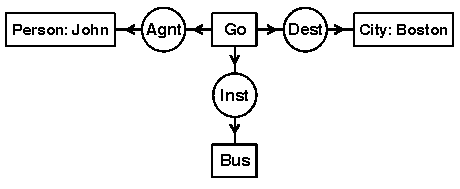
\includegraphics[scale=0.6]{./img01/graf.png} 
\caption{Przyk�ad grafu konceptualnego.}
\label{fig:graf_konceptualny}
\end{figure} 
 
Jak podaje wiele �r�de�\textbf{[jakie �r�d�a?]} grafy konceptualne s� bardzo wygodnym narz�dziem pozwalaj�cym na przetwarzanie j�zyka naturalnego. Potwierdza to powy�szy graf prezentuj�cy wiedz� ze zdania ,,John jedzie autobusem do Bostonu'', pochodz�cego z j�zyka naturalnego.\\
Taki spos�b reprezentacji wiedzy pozwala za pomoc� prostok�t�w przedstawia� istniej�ce obiekty lub zdarzenia z pewnego fragmentu opisywanej rzeczywisto�ci. Obiekty te, podobnie jak poprzednio, nazwane zosta�y konceptami lub poj�ciami. Natomiast okr�gi okre�laj� relacje zachodz�ce pomi�dzy tymi obiektami. W prezentowanym przyk�adzie \texttt{Agnt} oznacza gagenta czyli g��wnego wykonawc� czynno�ci, \texttt{Inst} okre�la narz�dzie wykorzystane przy danej czynno�ci oraz \texttt{Dest} okre�la jej cel.\\
Og�lna rzecz bior�c sieci semantyczne s�u�� do formalnej reprezentacji pewnego w�skiego fragmentu rzeczywisto�ci. W tym celu wykorzystuj� one dwa rodzaje obiekt�w. Pierwszym z nich s� koncepty reprezentuj�ce pewne fizyczne byty, atrybuty lub zdarzenia charakterystyczne dla opisywanej dziedziny. Natomiast drugi typ okre�la relacje wyra�aj�ce zale�no�ci mi�dzy obiektami. Zwi�zki mi�dzy obiektami mo�na okre�li� mianem semantyki graf�w konceptualnych. Opisywany j�zyk reprezentacji wykorzystuje r�wnie� elementy logiki, kt�re wyznaczaj� czy okre�lony koncept jest elementem opisywanej rzeczywisto�ci czy te� nie. W tym celu u�ywane s� kwantyfikatory: og�lny oraz egzystencjalny, a tak�e operatory: negacji, alternatywy i koniunkcji.
  
\subsection{Resource Description Framework}
RDF jest przyk�adem j�zyka o bardzo rygorystycznym stopniu formalizacji. J�zyk ten opracowany zosta� w celu stworzenia formalnego standardu daj�cego mo�liwo�� automatycznej interpretacji i przetwarzania wiedzy przez systemy komputerowe i wirtualnych agent�w. Warto doda�, i� standard ten opracowany zosta� przez konsorcjum W3C.\\
Reprezentacja ontologii przy pomocy RDF wymaga u�ycia pewnego formalnego sposobu zapisu danych. W tym celu wykorzystuje si� tzw. metaj�zyki. Jedna z najprostszych definicji okre�la metaj�zyki jako: ,,j�zyki s�u��ce do definiowania innych j�zyk�w'' \cite{Sem}. Jednym z najpopularniejszych i cz�sto stosowanych metaj�zyk�w jest XML. Jest to j�zyk bazuj�cy na znacznikach pozwalaj�cy na reprezentacj� danych w postaci specjalnie zdefiniowanej struktury. Obecnie wi�kszo�� j�zyk�w lub standard�w s�u��cych do opisu ontologii zbudowanych jest w�a�nie na bazie XML.\\ 
G��wna idea RDF zak�ada mo�liwo�� opisu pewnego bardzo w�skiego fragmentu rzeczywisto�ci w postaci tzw. tr�jek lub tryplet�w. Zaliczamy do nich:
\begin{itemize}
\item podmiot/klasa - okre�la zasoby czyli pewne obiekty lub zdarzenia wyst�puj�ce w modelowanej dziedzinie,
\item predykat - mo�e by� interpretowany jako pewne w�asno�ci lub atrybuty danego obiektu,
\item obiekt - jest to warto�� danego predykatu lub inaczej warto�� okre�lonego atrybutu obiektu.
\end{itemize}
Warto doda�, i� j�zyk RDF posiada bardzo ciekawy mechanizm identyfikacji tryplet�w. W tym celu wykorzystuje on standard URI (Uniform Resource Identifier). URI jest standardem wykorzystywanym do identyfikacji zasob�w w sieciach komputerowych.

Jak wspomniano wcze�niej RDF, jest j�zykiem bazuj�cym na j�zyku znacznik�w XML. Pozwala to na reprezentacj� wiedzy w postaci struktury drzewiastej. RDF posiada niezwykle u�yteczny mechanizm dziedziczenia umo�liwiaj�cy praktycznie nieograniczon� mo�liwo�� rozszerzania klas oraz predykat�w. W tym celu stosuje si� polecenia ,,rdfs:subClassOf'' oraz ,,rdfs:subPropertyOf''.

W kontek�cie j�zyka RDF warto w kilku zdaniach odnie�� si� do standardu RDF Schema. RDFS jest j�zykiem reprezentacji wiedzy opartym na RDF. Nie definiuje on nowych poj�� ale tworzy struktury zwane s�ownikami RDF. S� to r�nego rodzaju mechanizmy s�u��ce do opisu klas oraz predykat�w (w�a�ciwo�ci, atrybut�w). Dzi�ki RDFS mo�liwe jest zdefiniowanie zbioru klas i predykat�w stosowanych ��cznie do opisu okre�lonego obiektu czy mechanizm hierarchizacji klas. Definiuj�c w tym j�zyku klas� Samoch�d, mo�na j� zdefiniowa� jako klas� podrz�dn� klasy pojazd ko�owy, kt�ra stanowi podklas� klasy pojazd. Ta w�asno�� sprawia, �e RDFS jest j�zykiem bardzo zbli�onym do obiektowych j�zyk�w programowania. Ponadto RDFS umo�liwia tworzenie zale�no�ci pomi�dzy klasami oraz predykatami, co znacznie usprawnia mechanizm wnioskowania na podstawie dostaczonej bazy wiedzy. Na koniec warto wspomnie� i� RDF Schema stanowi baz� dla j�zyka OWL. 

\subsection{Ontology Web Language}
Ostatnim prezentowanym przyk�adem j�zyka stosowanego do formalnej reprezentacji ontologii jest j�zyk OWL. Stanowi on rozszerzenie j�zyk�w RDF i RDF Schema. Nale�y on do j�zyk�w o bardzo wysokim stopniu formalizacji. Oznacza to, �e taki spos�b reprezentacji wiedzy umo�liwia jej interpretacj� oraz automatyczne przetwarzanie przez systemy komputerowe lub wirtualnych agent�w. Podobnie jak RDF, standard ten, zosta� opracowany przez konsorcjum W3C.

Sk�adnia j�zyka OWL jest zgodna ze standardem XML, natomiast jego semantyka bazuje na tzw. logice opisowej. Najpro�ciej definiuj�c terminem logiki opisowej mo�na okre�li� zbi�r j�zyk�w reprezentacji ontologii, umo�liwiaj�cych (w r�nym stopniu) przeprowadzenie procesu wnioskowania. Ponadto OWL jest znacznie bardziej rozbudowany ni� RDF czy RDFS, gdy� posiada bogatsz� sk�adni� s�u��c� do budowy klas, przypisywania im okre�lonych w�asno�ci, definiowania ich wzajemnej relacji, a tak�e posiada metody pozwalaj�ce na reprezentacj� tego samego fragmentu rzeczywisto�ci przy pomocy r�nych wersji ontologii. Warto wspomnie�, i� istniej� 3 r�ne odmiany tego j�zyka, charakteryzuj�cych si� r�nym stopniem funkcjonalno�ci. Wyr�nia si�:
\begin{itemize}
\item OWL Lite - ograniczenia w stosunku do konstruktor�w tego j�zyka (brak klas wyliczeniowych czy roz��czno�ci), �atwo�� implementacji, ograniczona ekspresyjno��,
\item OWL DL - mniejsze ograniczenia konstruktor�w j�zyka, zapewnia efektywne wnioskowanie, utrata kompatybilno�ci z RDF
\item OWL Full - dost�pno�� wszystkich konstrukcji j�zyka OWL, mo�liwo�� wykorzystywania konstrukcji z j�zyk�w RDF i RDFS, ograniczone wsparcie dla mechanizmu wnioskowania.
\end{itemize}     
\subsection{Podsumowanie}
W niniejszym rozdziale przedstawiono kilka wybranych formalnych metod reprezentacji ontologii. Nosz� one nazw� j�zyk�w reprezentacji. Jednym z najwa�niejszych kryteri�w podzia�u tych j�zyk�w jest stopie� formalizacji. Jego stopie� okre�la stopie� formalizacji semantyki. Im wy�szy stopie� formalizacji tym wi�ksza podatno�� reprezentacji na jej automatyczne przetwarzanie przez programy komputerowe. Niestety taki spos�b przedstawiania wiedzy jest bardzo nieczytelny dla ludzi. Niski stopie� formalizacji zwi�zany jest z j�zykiem naturalnym u�ywanym przez ludzi. Ze wzgl�du na spor� liczb� niejasno�ci oraz tendencji do dwuznaczno�ci nie nadaje si� on do komputerowego przetwarzania.\\
Wsp�ln� cech� wielu j�zyk�w reprezentacji jest spos�b reprezentacji ontologii w postaci, tzw. tryplet�w czyli klas, predykat�w (w�asno�ci lub atrybut�w) klas oraz warto�ci tych atrybut�w wraz z ograniczeniami. Zalet� takiego sposobu reprezentacji jest stosunkowo du�a �atwo�� dokonywania zmian, a tak�e mo�liwo�� jej wielokrotnego przetwarzania w przypadku r�nych zada�.

\section{Cel projektu}
\label{sec:druga}
Celem projektu jest wykorzystanie dost�pnej bazy wiedzy dotycz�cej wyspecjalizowanej dziedziny, w tym wypadku informacji opisuj�cych r�ne style piwa. Baza wiedzy, znaleziona przy pomocy \emph{Swoogle}, zosta�a wykorzystana jako zestaw poj�� do opisu ww. dziedziny. Dysponuj�c tym modelem, mo�na wykorzysta� go, importuj�c do w�asnej bazy wiedzy, kt�ra na tej podstawie opisuje w�asne instancje. Zalet� takiego rozwi�zania jest stworzenie architektury rozproszonej. Baza g��wna mo�e znajdowa� si� w dowolnym miejscu w sieci, wystarczy, �e b�dzie dost�pna. Wykorzystuj�c t� baz�, dowolna firma produkuj�ca piwo, b�dzie w stanie na jej podstawie stworzy� w�asn� baz�, opisuj�c� w�asne wyroby, tworz�c instancje danych styl�w piwa.
Dysponuj�c potrzebnymi elementami, czyli s�ownikiem oraz bazami firmowymi, wykorzystuj�cymi ten s�ownik, mo�na przyst�pi� do wykorzystania tych rozproszonych informacji w jednym miejscu. 

Projekt ten mo�na zrealizowa� na dwa sposoby. Pierwszym sposobem jest wykorzystanie zapyta� w j�zyku SPARQL z poziomu programu i w ten spos�b uzyskiwa� potrzebne o w�a�ciwo�ciach poszczeg�lnych styl�w piwa oraz ich instancjach. Podej�cie to, nie wymaga pobierania tych baz do pami�ci komputera, gdy� zapytanie zwraca jedynie wymagane informacje. Mo�na r�wnie� dokona� agregacji poszczeg�lnych graf�w reprezentuj�cych bazy wiedzy do jednej struktury grafowej w programie. Do wykonania takiej operacji s�u�y Apache Jena - framework napisany w j�zyka Java. Dopiero na tej zintegrowanej strukturze mo�na odczytywa� potrzebne informacje.

\section{Narz�dzia}
\label{sec:narzedzia}
W celu realizacji wybranego zadania projektowego wykorzystano nast�puj�ce narz�dzia:
\begin{itemize}
\item Protege(\url{www.http://protege.stanford.edu/}) -- edytor s�u��cy do tworzenia ontologii,
\item Apache Jena (\url{www.http://jena.apache.org/}) -- jest to API umo�liwiaj�ce operowanie na bazach wiedzy, ich agregacj�, wy�wietlanie potrzebnych informacji,
\item Swoogle (\url{www.http://swoogle.umbc.edu/}) - wyszukiwarka pozwalaj�ca na znalezienie dokument�w semantycznego Weba na podstawie s��w kluczowych; dodatkowo z dokument�w tych wyodr�bniane s� metadane co s�u�y do okre�lenia relacji mi�dzy nimi.\cite{Sem}.
\end{itemize} 

\section{Semantic Beer Base}
W ramach projektu powsta� program Semantic Beer Base, kt�ry umo�liwia wczytywanie s�ownika oraz baz firmowych zawieraj�cych instancje r�nych styl�w piwa. Program, za pomoc� Jeny ��czy poszczeg�lne bazy firmowe w jeden graf, a nast�pnie wy�wietla wszystkie te instancje, dodaj�c w�a�ciwo�ci reprezentowanego przez nie stylu piwa. Informacje te wy�wietlane s� za pomoc� struktury drzewiastej. Przyk�ad dzia�ania aplikacji, wy�wietlaj�cej wczytane informacje przedstawione zosta�y na rys. 

Program wy�wietla instancje piw ontologii firmowych i dla ka�dej z nich dodaje nazw� stylu kt�ry reprezentuje dana instancja. Mo�liwe jest r�wnie� wy�wietlenie atrybut�w zwi�zanych z danym stylem. W tym przypadku s� to sk�adniki, z kt�rych mo�na uwarzy� piwo w danym stylu. Informacje te pobierane s� z g��wnej ontologii, a dok�adniej, jest to, wspomniany ju� wcze�niej, atrybut ,,madeFrom''.


\bibliography{bibliografia01}
\addcontentsline{toc}{section}{Bibliografia}


\end{document}